% !TEX root = ../main.tex
%% Section 4: LLM-GridEval Framework

\section{LLM-GridEval Framework}\label{sec:framework}

\subsection{Framework Architecture}\label{sec:architecture}

LLM-GridEval integrates the system model into a unified evaluation environment through three layers (Fig.~\ref{fig:architecture}): a co-simulation layer, an interface and tool layer, and a cognitive layer.
The co-simulation layer implements the physical plant through a HELICS federation with five time-synchronized federates: a GridPACK transmission federate (IEEE 9-bus), two GridLAB-D distribution federates (IEEE 123-node feeders, with Feeder~A containing EV loads), a feeder controller federate implementing the defensive policy, and an MCP attacker server federate that bridges the interface layer.
The interface and tool layer acts as a sandboxed API boundary between the co-simulation and the attacker, implemented as a FastAPI HTTP server wrapping a HELICS federate; each attack primitive is defined by a JSON schema specifying inputs, outputs, preconditions, and the mapping to HELICS operations, and the layer performs argument validation and constraint enforcement (capacity bounds, cooldown timers, ramping rate limits) before invoking HELICS calls, ensuring that all actions issued by any attacker (including a fully autonomous LLM) are physically realizable and auditable.
The cognitive layer hosts the attacker policy $\pi$ using a ReAct-style interaction loop: (1)~observe grid state via \texttt{get\_grid\_status()}, (2)~assess timing via macro and micro scoring, (3)~query the LLM for an action specification, (4)~validate the response against the primitive schema, (5)~execute via the sandboxed interface, and (6)~advance the simulation clock.
This layered separation enables controlled experimentation: researchers can swap attacker implementations (scripted baselines, RL agents, or LLM-based policies) while keeping the co-simulation and tool interface fixed, isolating the impact of policy changes on measured outcomes.

\begin{figure}[t]
  \centering
  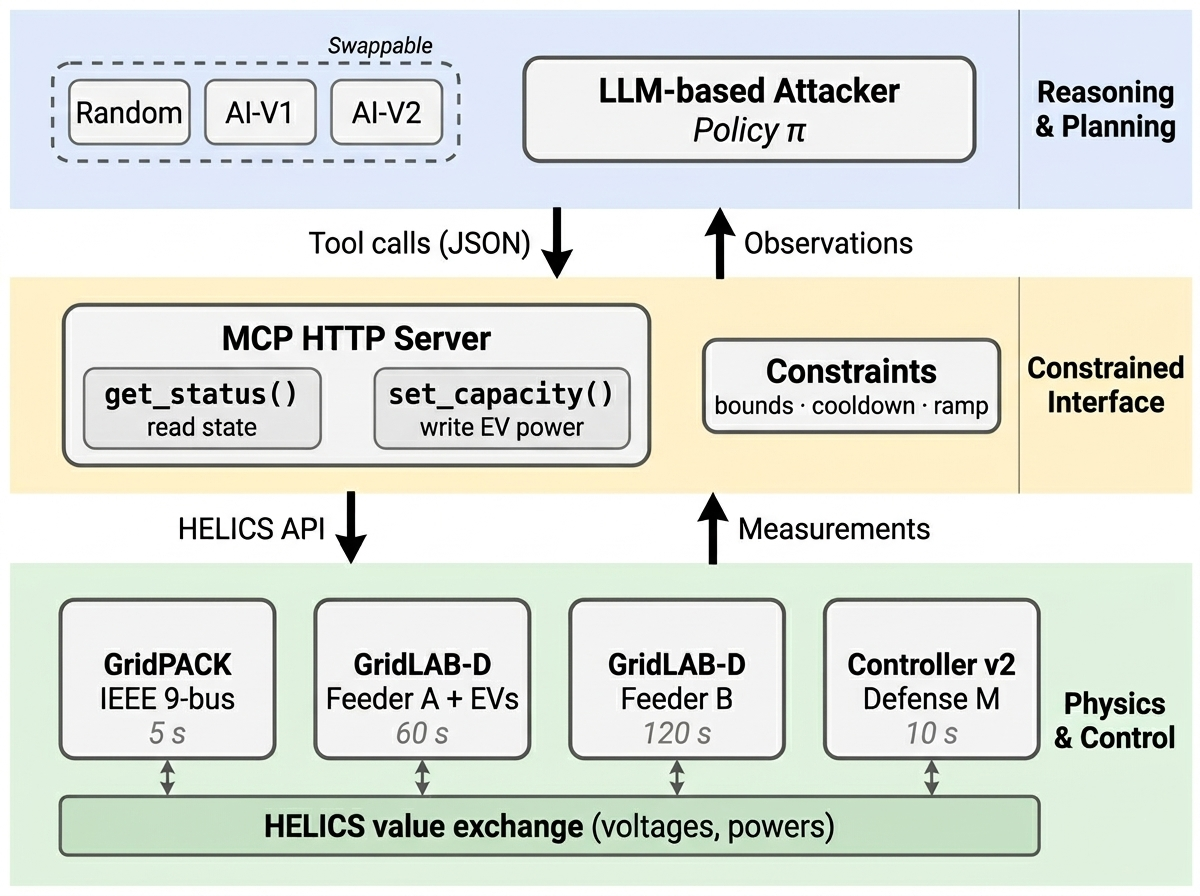
\includegraphics[width=\columnwidth]{figures/figure_added.png}
  \caption{LLM-GridEval architecture. The co-simulation layer (bottom) runs the HELICS federation; the interface layer (middle) enforces schema-constrained primitives with validation; the cognitive layer (top) hosts swappable attacker policies.}
  \label{fig:architecture}
\end{figure}

\subsection{Progressive-Shedding Controller (Blue Team)}\label{sec:controller}

The defender is a state-machine-based feeder controller (v2) that polls total feeder power at the swing node every 10 seconds and operates in four states.
In the \textsc{Overload} state ($P_{\text{feeder}} \geq 4200$~kW), the controller sheds one active EV per 10-second observation cycle in a randomized order that varies per experiment seed, requiring $N$ controller cycles to shed $N$ simultaneously active EVs---a property that makes target diversification strategically significant for attackers.
In the \textsc{Caution} state ($2600 < P < 4200$~kW), the controller maintains EV1 and EV2 at nominal power while shedding EV3--EV6; in the \textsc{Recovery} state ($P \leq 2600$~kW), it restores one previously shed EV per 30-second holdoff period.
In the \textsc{Normal} state ($P_{\text{feeder}} \leq 2600$~kW and all EVs active), no action is taken.
This controller represents a realistic baseline congestion management mechanism; commands arrive immediately with no message delay (correcting a critical 3600-second delay bug in the v1 prototype that rendered the controller non-functional during experiments).

\subsection{Attacker Variants (Red Team)}\label{sec:attackers}

We evaluate three attacker policies through the same MCP primitive interface, ensuring that observed differences in outcomes reflect policy quality rather than interface advantages.
The random baseline ($\pi_{\text{static}}$) represents a static, non-adaptive policy: at each 5-second observation interval, if the 90-second cooldown has elapsed, it attacks with probability $P = 0.3$, selecting the target EV uniformly from \{EV1, \ldots, EV6\} and power uniformly from [500, 1500]~kW, with no awareness of grid state, controller timing, or attack history.
The random baseline has the same interface access as the adaptive variants (including \texttt{get\_grid\_status()}) but does not use observations, serving as a simple non-adaptive comparator.
AI-V1 ($\pi_{\text{adapt}}^{(1)}$) uses Qwen~3.5-122B (a mixture-of-experts thinking model with 122B total and 10B active parameters) with a timing gate that pre-filters observations before LLM invocation: the LLM is called only when the micro-timing score exceeds 70 (indicating the controller just acted, leaving a $\geq$7-second window) and the cooldown has elapsed; the system prompt provides timing score interpretation but includes no information about the power accumulation model, no diversification guidance, and no attack history.
AI-V2 ($\pi_{\text{adapt}}^{(2)}$) extends V1 with explicit domain knowledge injected into the system prompt: an explanation that EV power contributions are additive across distinct targets but overwrite when the same EV is re-attacked, a priority instruction to attack unmodified EVs before repeating any target, and dynamic per-call context showing which EVs have been attacked and their current power levels---identical model, identical interface, identical constraints, different prompt content.
This power accumulation model---where $P_{\text{total}} = P_{\text{base}} + \sum_{i=1}^{6} P_{\mathrm{EV}_i}$ with overwrite semantics on same-EV re-attacks---means that three attacks on EV1 at 1500~kW contribute only 1500~kW total, while three attacks on EV1, EV2, and EV3 at 1500~kW each contribute 4500~kW, making target diversification essential for effective load accumulation.

\begin{table*}[t]
  \caption{Attacker variant comparison. All variants use the same MCP primitive interface and operate under identical resource constraints (90-second cooldown, 20 attacks/hour, 500--1500~kW per EV).}\label{tab:variants}
  \centering
  \small
  \begin{tabular}{@{}lcccc@{}}
    \toprule
    \textbf{Property} & \textbf{Random ($\pi_{\text{static}}$)} & \textbf{AI-V1 ($\pi_{\text{adapt}}^{(1)}$)} & \textbf{AI-V2 ($\pi_{\text{adapt}}^{(2)}$)} \\
    \midrule
    Timing intelligence   & None             & Micro-timing gate       & Micro-timing gate \\
    Domain knowledge      & None             & None                    & Power accumulation model \\
    Target selection      & Uniform random   & LLM (no context)        & LLM + diversification priority \\
    Power selection       & $\mathcal{U}$[500,\,1500] kW & LLM (no guidance) & Fixed 1500 kW (max) \\
    Attack history        & None             & None                    & Dynamic per-call context \\
    \bottomrule
  \end{tabular}
\end{table*}

\subsection{LLM Orchestration Details}\label{sec:orchestration}

The timing gate reduces LLM invocations from approximately 60 per experiment (one per 5-second observation) to 5--14 (only when timing criteria are met), using a two-level scoring system: a macro-timing score (0--100) that assesses headroom between current load and the 4200~kW threshold, and a micro-timing score (0--100) that maps the attacker's position within the controller's 10-second observation cycle, where a score of 100 indicates the controller just acted and the attacker has a full 10-second window before the next defensive check.
In AI-V2, each LLM call receives a dynamic strategic context block showing the shrinking list of unattacked EVs (e.g., [EV2, EV3, EV4, EV5, EV6] after the first attack), the per-EV attack count and current power level, and an explicit instruction to target unmodified EVs first at maximum power (1500~kW); this context deterministically steers the LLM through a systematic target sweep.
All LLM-based experiments use Qwen~3.5-122B-A10B (AWQ 4-bit quantization) served via vLLM, with temperature 0.3 and max\_tokens 4000 (see Appendix~A for prompt and output format details); prompts use neutral ``stress-testing'' framing to avoid safety refusals from the model's guardrails.
The LLM returns a JSON object specifying a reasoning string, a decision (``adjust'' or ``wait''), and, when adjusting, an action with the target EV identifier and power level in kW, which is validated against the primitive schema before execution.
